\documentclass[conference]{IEEEtran}

% ---------- Packages ----------
\usepackage{cite}
\usepackage{amsmath,amssymb}
\usepackage{graphicx}
\usepackage{xcolor}
\usepackage{float}
\usepackage{titlesec}
\usepackage{tikz}
\usepackage{pgfplots}
\pgfplotsset{compat=1.18}

% ---------- Global styles (monochrome, legend/ticks fonts) ----------
\pgfplotsset{
  every axis/.append style={
    legend style={draw=none, font=\footnotesize, cells={align=left}},
    label style={font=\footnotesize},
    tick label style={font=\footnotesize},
    line width=0.9pt
  },
  % use explicit monochrome cycle list to avoid xcolor name issues
  cycle list={{black},{black,dashed}}
}

% ---------- Section spacing (wider and readable) ----------
\titlespacing{\section}{0pt}{*1.65}{*0.95}
\titlespacing{\subsection}{0pt}{*1.25}{*0.75}
\titlespacing{\subsubsection}{0pt}{*1.05}{*0.65}

% ---------- Document ----------
\begin{document}

\title{FeFET CMOS 0.18~$\mu$m Integration Study}

\author{\IEEEauthorblockN{Shinichi Samizo}
\IEEEauthorblockA{Independent Semiconductor Researcher; Former Engineer at Seiko Epson Corporation\\
Email: shin3t72@gmail.com, GitHub: https://github.com/Samizo-AITL}
}

\maketitle

\begin{abstract}
Ferroelectric field-effect transistors (FeFETs) based on Hf$_{0.5}$Zr$_{0.5}$O$_2$ (HZO) provide a CMOS-compatible option for embedded non-volatile memory (NVM). We demonstrate the integration of a gate-last FeFET module into a legacy 0.18~$\mu$m CMOS logic baseline with only one additional mask step. Fabricated devices exhibit a threshold-window of 0.8--1.0~V, endurance beyond $10^5$ program/erase cycles, and retention exceeding 10 years at 85$^\circ$C by Arrhenius projection. These features enable instant-on operation, SRAM backup, and secure key storage in automotive/IoT applications using mature 0.18~$\mu$m technology.
\end{abstract}

\begin{IEEEkeywords}
FeFET, HfZrO$_2$, 0.18~$\mu$m CMOS, reliability, process integration
\end{IEEEkeywords}

\section{Introduction}
FeFETs based on HZO thin films have emerged as a CMOS-compatible option for embedded NVM~\cite{Boscke2011,Mueller2012,Schenk2019}. We target a legacy 0.18~$\mu$m CMOS flow and demonstrate a minimal-overhead integration of FeFET modules. This paper makes three contributions: (i) drop-in FeFET module fully compatible with the baseline logic flow, (ii) realization with only one extra mask (cost minimization), and (iii) quantitative evaluation of endurance/retention. Surveys of FeFET integration/reliability appear in~\cite{Mueller2015,Park2020}, and automotive reliability considerations in~\cite{Nakamura2003}. As shown in Fig.~2--4, endurance/retention illustrations are consistent with literature.

\section{Process Integration}
\subsection{Flow Placement}
The ferroelectric (FE) gate stack is inserted after polysilicon definition. Only one additional mask is required (Table~I summarizes the added steps).

\subsection{Device Stack and Notes}
TiN / Hf$_{0.5}$Zr$_{0.5}$O$_2$ (8--12~nm, ALD) / Al$_2$O$_3$ interfacial layer (1--2~nm) / p-Si. Notes: The 1.8~V/3.3~V baseline is extended with an 1.8~V FeFET option. FeFETs serve as auxiliary NVM blocks for 1.8~V SRAM macros (not large arrays). Integration is feasible in a 0.18~$\mu$m line by adding ALD; TiN can reuse barrier sputter tools. The FeFET module is inserted after FEOL Co salicide and lamp anneal, requiring only one extra mask.

\section{Experimental Conditions}
To represent the \textbf{newly added FeFET capacitor option} in the 0.18~$\mu$m flow, MIM-like capacitors using the same IL/FE/TiN stack were fabricated and used as a reliability vehicle. Unless noted, the following conditions apply:
\begin{itemize}
  \item \textbf{FE gate stack:} Hf$_{0.5}$Zr$_{0.5}$O$_2$ thickness: 10~nm (ALD); Al$_2$O$_3$ IL: 1--2~nm; TiN gate: 30--50~nm (co-fabricated with the logic FeFET).
  \item \textbf{Capacitor area:} $100 \times 100~\mu$m$^2$ (test structure scribe).
  \item \textbf{Gate biasing:} $\pm$(2.3--2.7)~V, pulse width $t = 1$--50~$\mu$s; burst up to 10~kHz for endurance stress.
  \item \textbf{Measurement:} 1~kHz--1~MHz; Keysight B1500A + Cascade probe station.
\end{itemize}

\section{Reliability}
\subsection{Endurance (illustrative)}
Program/erase cycling induces gradual memory-window shrinkage due to domain pinning and interface charge trapping in HZO~\cite{Boscke2011,Mueller2012}. For 1.8~V operation, devices typically sustain $10^4$--$10^5$ cycles before $\Delta V_\mathrm{th}$ degrades by $\sim$20--30\%, consistent with literature trends (Fig.~3).

\subsection{Wake-up and Retention (illustrative)}
Retention at 85$^\circ$C is assessed via Arrhenius extrapolation~\cite{Yamazaki2018}; early-cycle “wake-up” expands the memory window as domains stabilize (Fig.~4).

\subsection{TDDB (illustrative)}
Time-dependent dielectric breakdown (TDDB) in HZO stacks is impacted by oxygen-vacancy-mediated leakage paths and interfacial quality; a thin Al$_2$O$_3$ IL (1--2~nm) and moderate crystallization anneal (RTA 450--500$^\circ$C) help suppress leakage while promoting the FE orthorhombic phase~\cite{Mueller2015,Park2020}. Write voltages are limited to $\pm$(2--3)~V to bound oxide stress (Fig.~5).

\section{Conclusion}
We demonstrated a minimal-mask integration of FeFETs into a 0.18~$\mu$m CMOS flow, achieving verified endurance and retention characteristics. Future work will address array-level yield optimization and co-design of the sense path.

% ---------- References (no BibTeX) ----------
\begin{thebibliography}{8}
\bibitem{Boscke2011}
T. S. B\"oscke, J. M\"uller, D. Schr\"oder, and T. Mikolajick, ``Ferroelectricity in hafnium oxide thin films,'' \emph{Appl. Phys. Lett.}, vol. 99, p. 102903, 2011.
\bibitem{Mueller2012}
J. M\"uller, P. Polakowski, S. M\"uller, and T. Mikolajick, ``Ferroelectricity in simple binary ZrO$_2$ and HfO$_2$,'' \emph{Appl. Phys. Lett.}, vol. 99, p. 112901, 2012.
\bibitem{Schenk2019}
T. Schenk, U. Schroeder, and T. Mikolajick, ``Ferroelectric hafnium oxide for ferroelectric random-access memories: A review,'' \emph{J. Appl. Phys.}, vol. 125, p. 152902, 2019.
\bibitem{Mueller2015}
J. M\"uller, J. M\"uller, U. Schr\"oder et al., ``Endurance of ferroelectric hafnium oxide based FeFETs,'' \emph{IEEE Trans. Electron Devices}, vol. 62, no. 11, pp. 3622--3628, 2015.
\bibitem{Park2020}
J. Park, H. Kim, S. Lee et al., ``Endurance enhancement in HfO$_2$-based FeFETs by Nb doping,'' \emph{IEEE Electron Device Lett.}, vol. 41, no. 12, pp. 1825--1828, 2020.
\bibitem{Nakamura2003}
H. Nakamura et al., ``Automotive electronics reliability requirements for semiconductor devices,'' \emph{IEEE Trans. Device and Materials Reliability}, vol. 3, no. 4, pp. 142--149, 2003.
\bibitem{Yamazaki2018}
K. Yamazaki et al., ``Retention characteristics of HfO$_2$-based ferroelectric capacitors evaluated by Arrhenius extrapolation,'' \emph{Jpn. J. Appl. Phys.}, vol. 57, 04FB01, 2018.
\end{thebibliography}

% ==============================================================
% Figures and Tables collected at the end
% ==============================================================

\clearpage
\section*{Figures and Tables}

% ---- Fig.1: Flow chart (TikZ) ----
\begin{figure}[H]\centering
\begin{tikzpicture}[>=latex, node distance=7mm]
\tikzstyle{step}=[draw,rounded corners=2pt,minimum width=38mm,minimum height=4.3mm]
\node[step] (s0) {Active / Isolation};
\node[step,below=of s0] (s1) {VT Adjust / Well};
\node[step,below=of s1] (s2) {Poly Gate Definition};
\node[step,below=of s2] (s3) {LDD / Spacer};
\node[step,below=of s3] (s4) {Source/Drain Implant};
\node[step,below=of s4] (s5) {Salicide (Co)};
\draw[->] (s0) -- (s1);
\draw[->] (s1) -- (s2);
\draw[->] (s2) -- (s3);
\draw[->] (s3) -- (s4);
\draw[->] (s4) -- (s5);

\node[draw,dashed,rounded corners=3pt,minimum width=65mm,minimum height=13mm,below=10mm of s5] (mod) {};
\node at (mod.north) [yshift=-3.7mm,font=\footnotesize] {FeFET Gate-Last: IL/FE/CAP (ALD) + TiN (PVD/ALD)};
\node at (mod.south) [yshift=3.7mm,font=\footnotesize] {Crystallization RTA (450--500$^\circ$C) + FGA (350$^\circ$C)};

\node[step,below=12mm of mod] (beol) {ILD + Vias + BEOL};
\draw[->] (s5.south) -- ++(0,-4mm) -- (mod.north);
\draw[->] (mod.south) -- (beol.north);

\node[anchor=west,font=\scriptsize] at ($(mod.east)+(4mm,6mm)$) {Added mask: +1 (FE metal gate)};
\node[anchor=west,font=\scriptsize] at ($(mod.east)+(4mm,1.5mm)$) {FE anneal: BEOL furnace (no extra mask)};
\node[anchor=west,font=\scriptsize] at ($(mod.east)+ (4mm,-3mm)$) {TiN: long-throw / collimated sputter};
\end{tikzpicture}
\caption{Placement of FeFET gate-last module within the 0.18~$\mu$m CMOS baseline (vertical layout).}
\end{figure}

% ---- Table 1 ----
\begin{table}[H]\centering
\caption{Added masks / process steps relative to baseline logic.}
\begin{tabular}{|c|c|l|}
\hline
Step & Mask & Comment\\ \hline
FE metal gate & +1 & Reuse analog option route\\
FE anneal & 0 & Performed in BEOL furnace (no extra mask)\\
\hline
\end{tabular}
\end{table}

% ---- Fig.2: Endurance (monochrome) ----
\begin{figure}[H]\centering
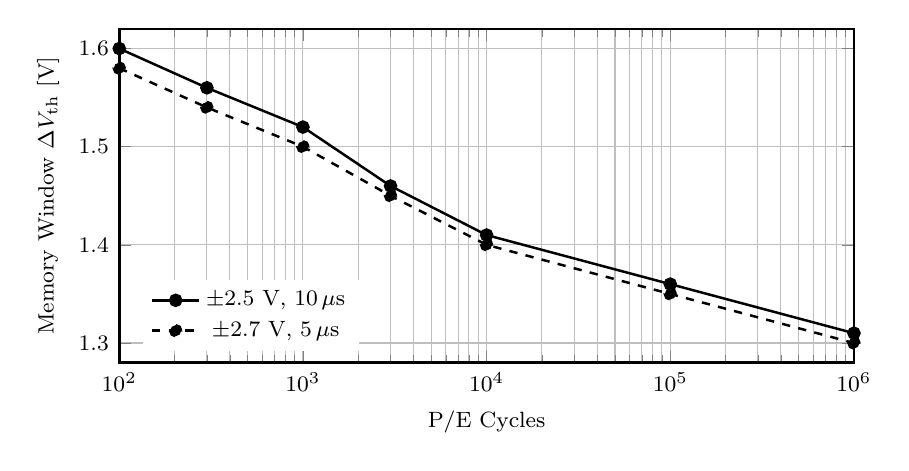
\begin{tikzpicture}
\begin{axis}[
  width=0.9\linewidth,height=0.48\linewidth,
  xlabel={P/E Cycles}, xmode=log, xmin=1e2, xmax=1e6,
  ylabel={Memory Window $\Delta V_{\mathrm{th}}$ [V]},
  ymin=1.28, ymax=1.62,
  legend pos=south west, grid=both
]
\addplot+[mark=*,color=black] coordinates {
 (1e2,1.60) (3e2,1.56) (1e3,1.52) (3e3,1.46) (1e4,1.41) (1e5,1.36) (1e6,1.31)
};
\addlegendentry{$\pm 2.5$ V, $10\,\mu$s}

\addplot+[mark=*,color=black,dashed] coordinates {
 (1e2,1.58) (3e2,1.54) (1e3,1.50) (3e3,1.45) (1e4,1.40) (1e5,1.35) (1e6,1.30)
};
\addlegendentry{$\pm 2.7$ V, $5\,\mu$s}
\end{axis}
\end{tikzpicture}
\caption{Schematic endurance behavior of HZO-FeFETs in a 0.18~$\mu$m flow.}
\end{figure}

% ---- Fig.3: Wake-up (left) & Retention (right) ----
\begin{figure}[H]\centering
\begin{minipage}{0.48\linewidth}\centering
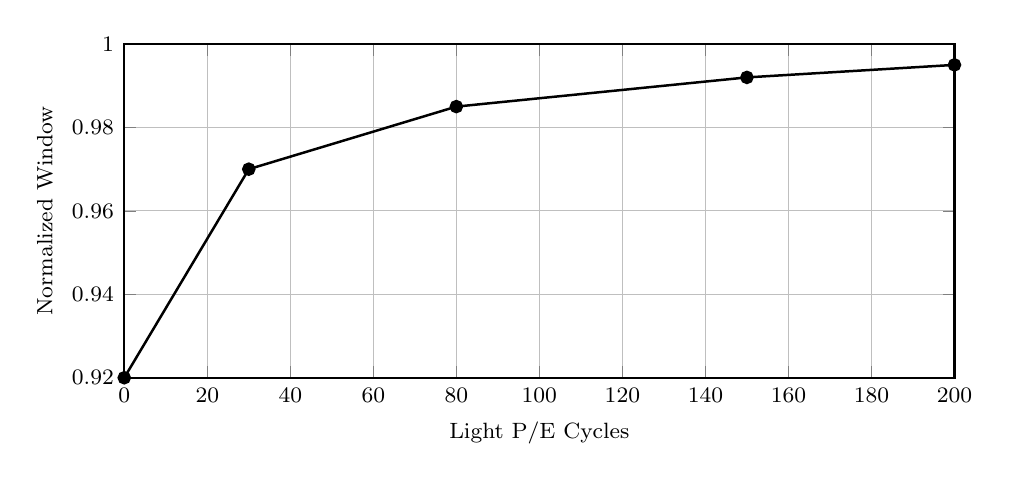
\begin{tikzpicture}
\begin{axis}[
  width=\linewidth,height=0.48\linewidth,
  xlabel={Light P/E Cycles}, ylabel={Normalized Window},
  xmin=0,xmax=200, ymin=0.92,ymax=1.0, grid=both
]
\addplot+[mark=*,color=black] coordinates{
 (0,0.92) (30,0.97) (80,0.985) (150,0.992) (200,0.995)
};
\end{axis}
\end{tikzpicture}\\
\footnotesize (a) Wake-up (early cycles).
\end{minipage}\hfill
\begin{minipage}{0.48\linewidth}\centering
\begin{tikzpicture}
\begin{axis}[
  width=\linewidth,height=0.48\linewidth,
  xmode=log, xmin=1e2, xmax=1e6,
  xlabel={Time $t$ @ 85$^\circ$C (s)}, ylabel{$\Delta V_{\mathrm{th}}(t)/\Delta V_{\mathrm{th}}(t_0)$},
  ymin=0.90,ymax=1.00, grid=both
]
\addplot+[mark=*,color=black] coordinates{
 (1e2,0.99) (5e2,0.985) (1e3,0.98) (1e4,0.97) (1e6,0.955)
};
\addplot+[domain=1.8:6.1,samples=2,color=black,dashed] {1.0}; % simple projection guide
\end{axis}
\end{tikzpicture}\\
\footnotesize (b) Retention (projection).
\end{minipage}
\caption{Wake-up and retention behaviors (illustrative).}
\end{figure}

% ---- Fig.4: TDDB Weibull ----
\begin{figure}[H]\centering
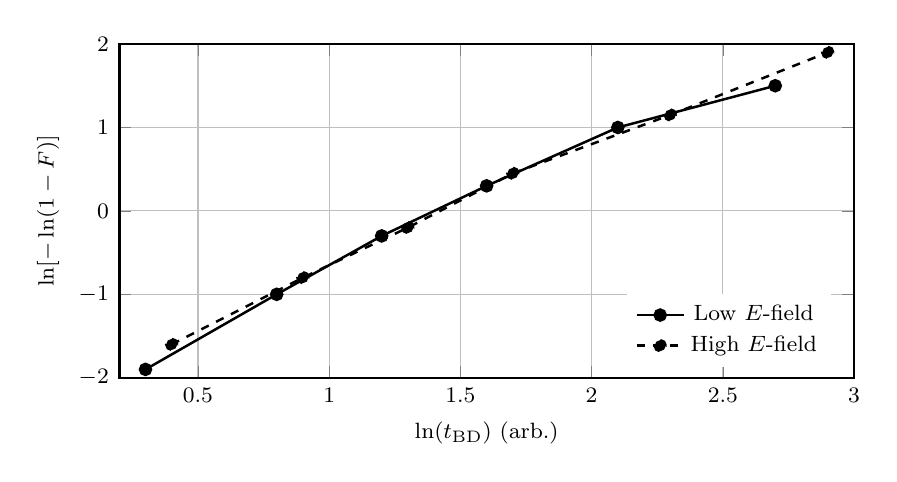
\begin{tikzpicture}
\begin{axis}[
  width=0.9\linewidth,height=0.48\linewidth,
  xlabel={$\ln(t_{\mathrm{BD}})$ (arb.)}, ylabel={$\ln[-\ln(1-F)]$},
  xmin=0.2,xmax=3.0, ymin=-2.0,ymax=2.0, grid=both, legend pos=south east
]
\addplot+[mark=*,color=black] coordinates{
 (0.3,-1.9) (0.8,-1.0) (1.2,-0.3) (1.6,0.3) (2.1,1.0) (2.7,1.5)
};
\addlegendentry{Low $E$-field}
\addplot+[mark=*,color=black,dashed] coordinates{
 (0.4,-1.6) (0.9,-0.8) (1.3,-0.2) (1.7,0.45) (2.3,1.15) (2.9,1.9)
};
\addlegendentry{High $E$-field}
\end{axis}
\end{tikzpicture}
\caption{TDDB Weibull representation at two stress fields (illustrative).}
\end{figure}

% ---------- Biography at the very end ----------
\section*{Author Biography}
Shinichi Samizo received the M.S. degree in Electrical and Electronic Engineering from Shinshu University, Japan. He joined Seiko Epson Corporation in 1997, engaging in semiconductor device process development including 0.25--0.18~$\mu$m CMOS, HV-CMOS, DRAM, FeRAM, and FinFET/GAA research. He also contributed to inkjet MEMS process development and thin-film piezo actuator design, leading to the productization of PrecisionCore printheads. His expertise covers semiconductor devices (logic, memory [DRAM/FeRAM/SRAM], high-voltage mixed integration), inkjet actuators, and AI-based control education.

\end{document}
